\documentclass{article}
\begin{document}
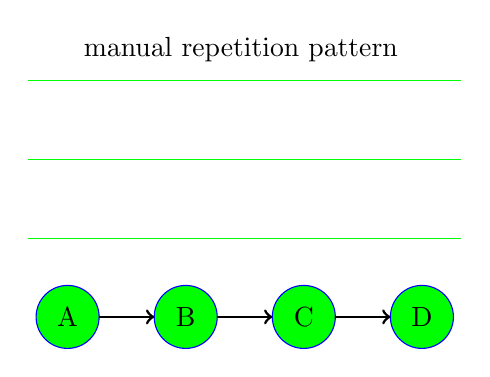
\begin{tikzpicture}
\foreach \x in {0,1.5,3,4.5} {
  \filldraw[draw=blue,fill=green] (\x,0) circle (0.4);
}
\node at (0,0) {A};
\node at (1.5,0) {B};
\node at (3,0) {C};
\node at (4.5,0) {D};
\draw[->,line width=1pt] (0.4,0) -- (1.1,0);
\draw[->,line width=1pt] (1.9,0) -- (2.6,0);
\draw[->,line width=1pt] (3.4,0) -- (4.1,0);
\foreach \y in {1,2,3} {
  \draw[green] (-0.5,\y) -- (5,\y);
}
\node at (2.2,3.4) {manual repetition pattern};
\end{tikzpicture}
\end{document}
